\chapter{Creating and Running Instances}
\par In this section we will add User accounts in keystone who can use Openstack System.
%Intro\footnotemark\\
\begin{spacing}{1.2}
%note en bas de page
\section{Creating a config for authentication}

\par We will connect with a user and create a configuration for the authentication of
Keystone. To do this, we will leave the root, then modify  / keystonerc and display the list
[flavor] available: 
\\
\begin{figure}[!htb] 
\begin{center} 
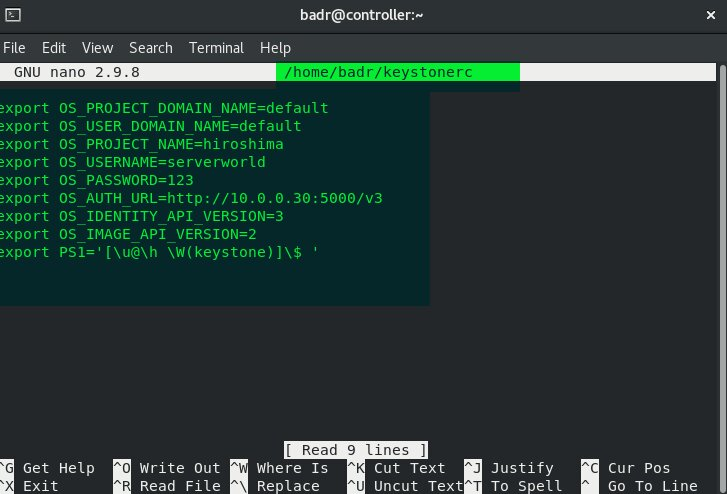
\includegraphics[width=1\linewidth]{Cloud/Creating and Running Instances/configuring environment variables} 
\end{center} 
\caption{configuring environment variables} 
\end{figure} 
\FloatBarrier
\\
\begin{figure}[!htb] 
\begin{center} 
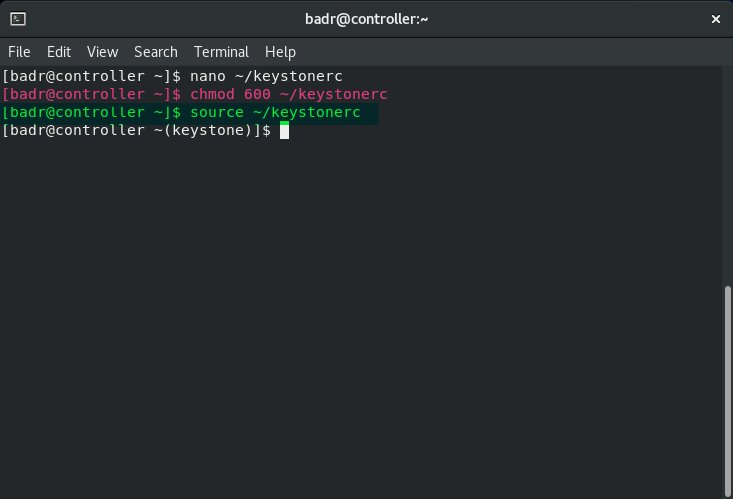
\includegraphics[width=1\linewidth]{Cloud/Creating and Running Instances/chmod and source} 
\end{center} 
\caption{chmod and source} 
\end{figure} 
\FloatBarrier
\\



\par Let's display the list of available images: 
\\
\begin{figure}[!htb] 
\begin{center} 
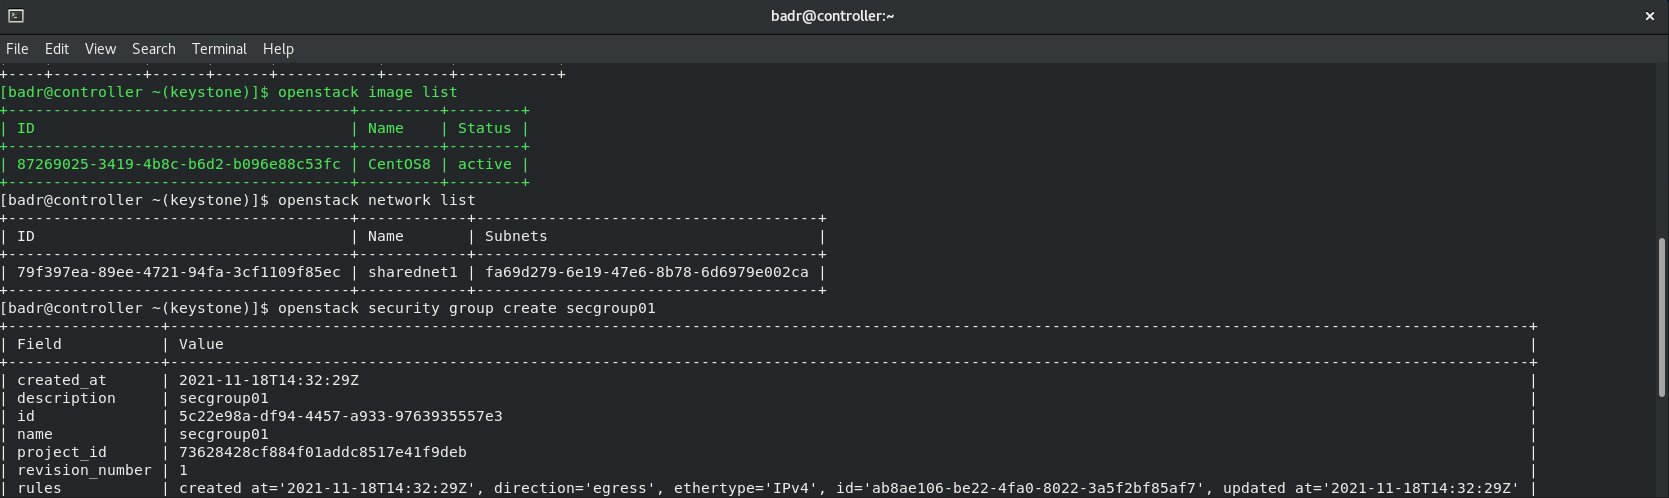
\includegraphics[width=1\linewidth]{Cloud/Creating and Running Instances/show available image list} 
\end{center} 
\caption{show available image list} 
\end{figure} 
\FloatBarrier

\par We will create a safety group for the instances:
\\
\begin{figure}[!htb] 
\begin{center} 
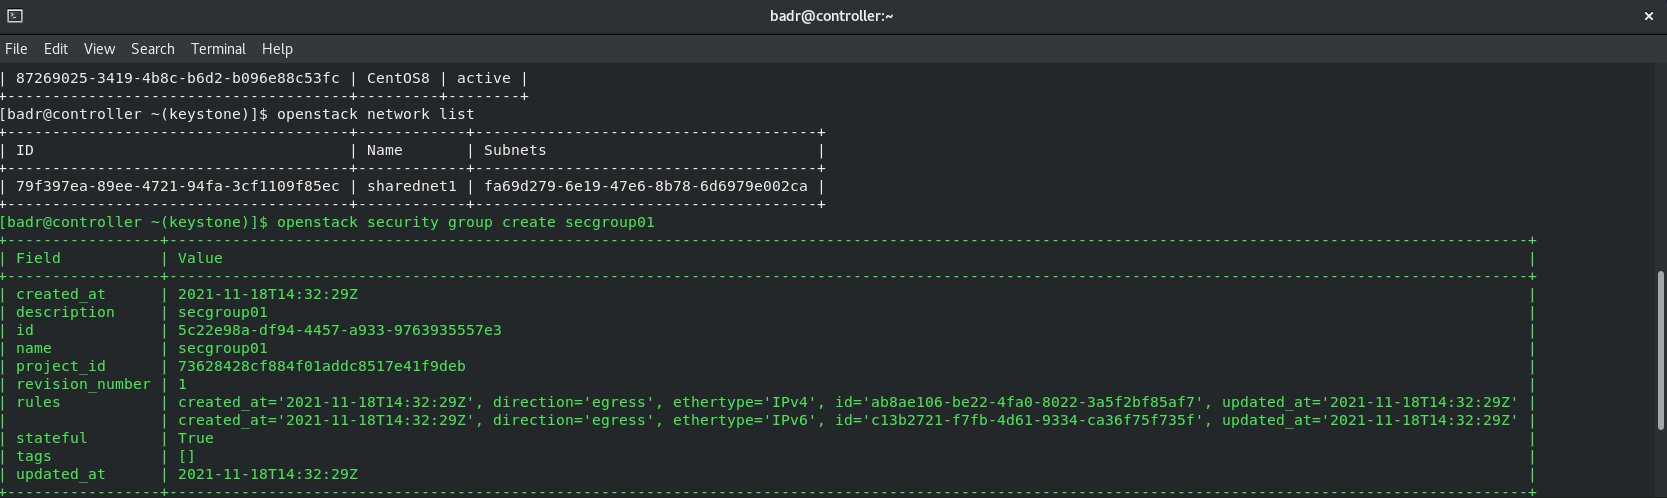
\includegraphics[width=1\linewidth]{Cloud/Creating and Running Instances/creating safety group} 
\end{center} 
\caption{creating safety group} 
\end{figure} 
\FloatBarrier

\\\par To verify this, we can display the list of security groups: 
\\
\begin{figure}[!htb] 
\begin{center} 
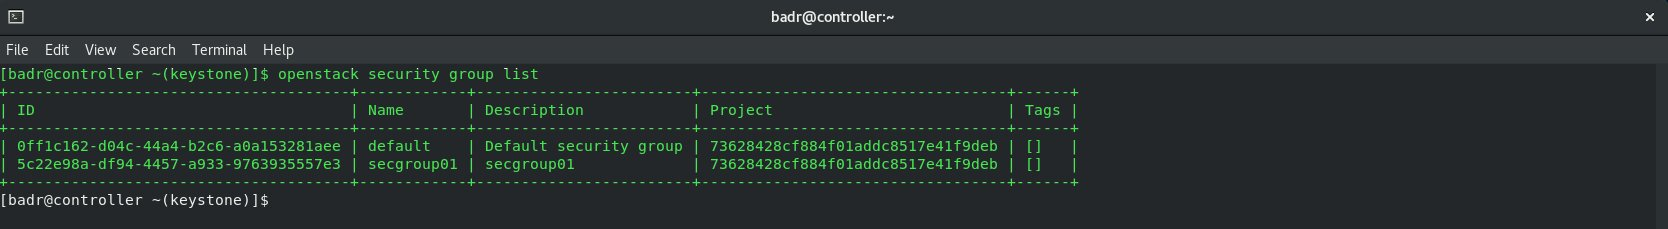
\includegraphics[width=1\linewidth]{Cloud/Creating and Running Instances/check security group} 
\end{center} 
\caption{check security group} 
\end{figure} 
\FloatBarrier
\\

\par Next, we will create an SSH key pair for connection to instances and add a key
public:
\\
\begin{figure}[!htb] 
\begin{center} 
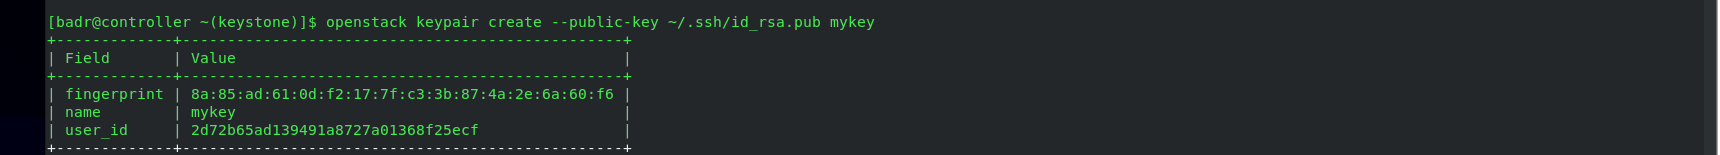
\includegraphics[width=1\linewidth]{Cloud/Creating and Running Instances/add public-key} 
\end{center} 
\caption{add public-key} 
\end{figure} 
\FloatBarrier
\\
\par We are ready to create and start an instance: 
\\
\begin{figure}[!htb] 
\begin{center} 
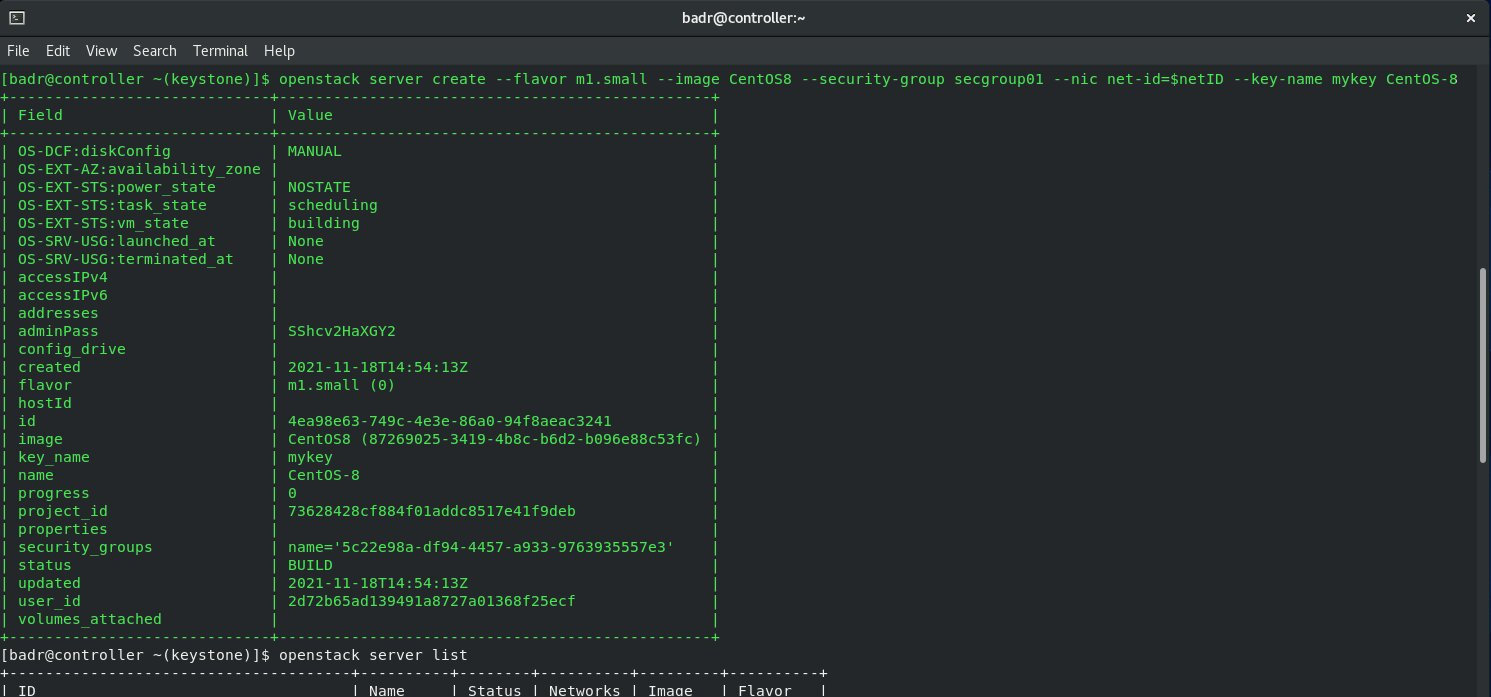
\includegraphics[width=1\linewidth]{Cloud/Creating and Running Instances/create and boot an instance} 
\end{center} 
\caption{create and boot an instance} 
\end{figure} 
\FloatBarrier
\\

\section{Configure security settings}





\par Now let's see the status the Openstack server.
\\
\begin{figure}[!htb] 
\begin{center} 
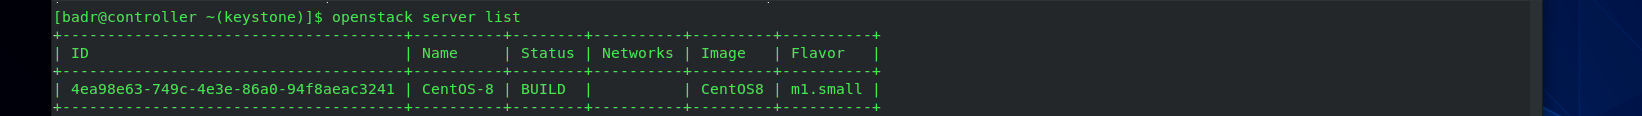
\includegraphics[width=1\linewidth]{Cloud/Creating and Running Instances/show status ([BUILD] status is shown when building instance)} 
\end{center} 
\caption{show status ([BUILD] status is shown when building instance)} 
\end{figure} 
\FloatBarrier
\\


\par Configuration for the security group you created above to access Internet Control Message Protocol.
\\
\begin{figure}[!htb] 
\begin{center} 
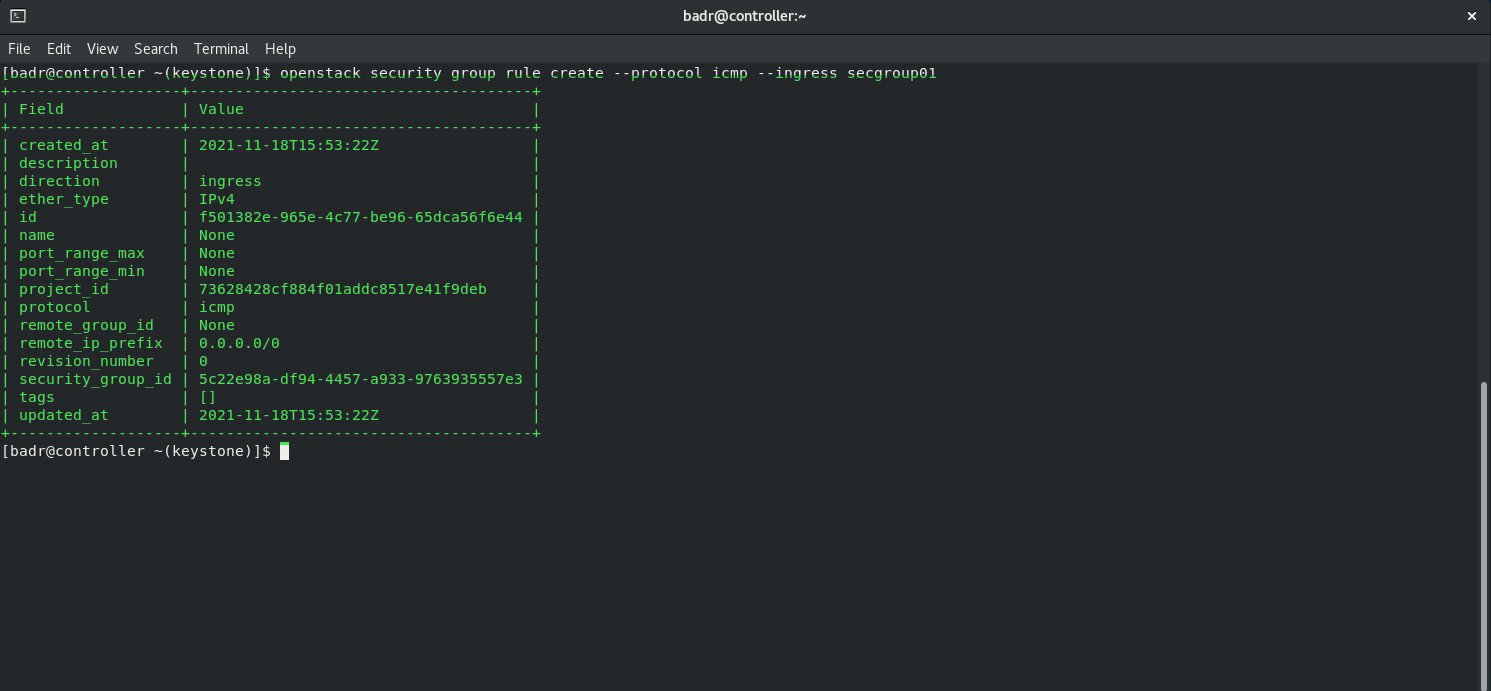
\includegraphics[width=1\linewidth]{Cloud/Creating and Running Instances/permit ICMP} 
\end{center} 
\caption{permit ICMP} 
\end{figure} 
\FloatBarrier
\\
\section{Login to the instance with SSH.}

\par Configuration for the security group you created above to access SSH.
\\
\begin{figure}[!htb] 
\begin{center} 
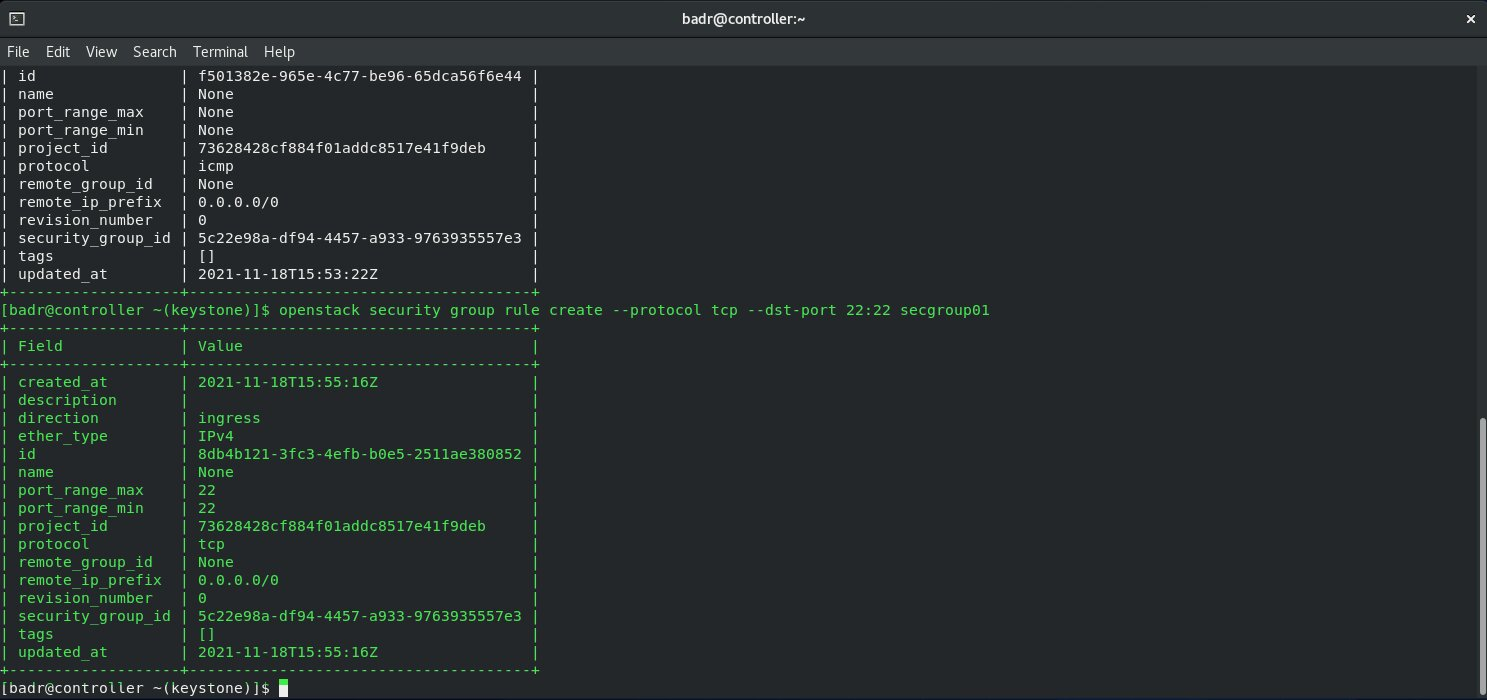
\includegraphics[width=1\linewidth]{Cloud/Creating and Running Instances/permit SSH} 
\end{center} 
\caption{permit SSH} 
\end{figure} 
\FloatBarrier
\\


\end{spacing}